\chapter{Set-membership identification}    % For a new chapter (works in book and report class)

Set-membership approach is an alternative to the classical, statistical identification approach. Least-Square method is one possible example of statistical estimation algorithms in the context of estimation.\\

\subsubsection{Main ingredients}

We consider a discrete-time system described in the following parametrized regression form:\\
\begin{equation}
y(k) = f(y(k-1), y(k-2), \cdots, y(k-n), u(k), u(k-1), \cdots, u(k-m), \theta_1, \theta_2, \cdots, \theta_{n+m+1})
\end{equation}

where \(m\leq n\)\\
A-priori information on the system:
\begin{itemize}
    \item \(n\) and \(m\) are known
    \item \(f \in \mathbb{F}\) where \(\mathbb{F}\) is the class of model selected on the basis of our physical insight. 
\end{itemize}


A-priori information on the noise, the main difference with respect to the previous discussion.
\begin{itemize}
    \item the noise structure is known, i.e. the way the way uncertainty affects the input-output data)
    \item the noise is assumed to belong to konwn bounded set \(\mathbb{B}\).
\end{itemize}

When the consistency property of LS was discussed, and in general statistical approach to system identification, the typicall assumption on the noise is that statistical distribution of the noise sequence, or the value of some moments of inertia of the noise is known, such as variance. Here, the assumption is that the noise sequence \(\eta\) belongs to a bounded \(\mathbb{B}\). Remember that assumption two of the consistency property was the crucial one, so a change of perspective is adopted on the second assumption, where we deal with the following problem:

\textbf{Set-membership identification of LTI system} under the assumption that the uncertainty affecting the data can be modelled as an equation error \(e(k)\), which is exactly assumption \(1\) considered for the consistency theorem.\\
\[
\begin{aligned}
\tilde{y}(k) = & -\theta_1 \tilde{y}(k - 1) - \theta_2 \tilde{y}(k - 2) - \cdots - \tilde{y}(k - n) \\[1ex]
               & + \theta_{n+1} \tilde{u}(k) + \theta_{n+2} \tilde{u}(k - 1) + \cdots + \theta_{n+m+1} \tilde{u}(k - m) + \mathbf{e(k)} \\[2ex]
\end{aligned}
\]
where,
\[
\begin{aligned}
e(k) \in \mathbb{B}e = \left\{ \bar{e} = [e(1), e(2), \cdots, e(H)]^T \right\} : \left| e(k) \right| \leq \Delta e, \forall k
\end{aligned}
\]
where  \(\Delta e \) is a given real bounded constant.

\begin{factbox}[]
In set-membership, we always have unknown and bounded assumption about the magnitude of noise.\\

The bound is considered a conservative bound.

\end{factbox}
\subsubsection{Error-in-Variable setting}
Let's assume that the data are actually collected from a real experiment, which is EIV setup. The block-diagram representation of this a-priori information is as follows.

\begin{center}
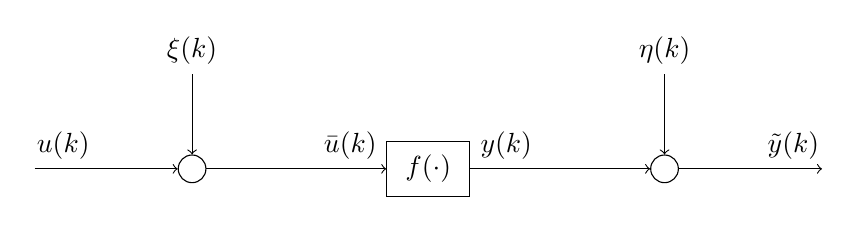
\begin{tikzpicture}[auto, node distance=2cm]

    % Block styles
    \tikzstyle{block} = [draw, rectangle, minimum height=2em, minimum width=3em]
    \tikzstyle{sum} = [draw, circle, inner sep=0pt, minimum size=1em]
    \tikzstyle{input} = [coordinate]
    \tikzstyle{output} = [coordinate]

    % Nodes
    \node [input] (input) {};
    \node [sum, right of=input, node distance=2cm] (sum1) {};
    \node [block, right of=sum1, node distance=3cm] (system) {$f(\cdot)$};
    \node [sum, right of=system, node distance=3cm] (sum2) {};
    \node [output, right of=sum2, node distance=2cm] (output) {};

    % Connections
    \draw [->] (input) -- node[pos=0.2] {$u(k)$} (sum1);
    \draw [->] (sum1) -- node[pos=0.8] {$\bar{u}(k)$} (system);
    \draw [->] (system) -- node[pos=0.2] {$y(k)$} (sum2);
    \draw [->] (sum2) -- node[pos=0.8] {$\tilde{y}(k)$} (output);
    
    % Noise terms
    \node [above of=sum1, node distance=1.5cm] (xi) {$\xi(k)$};
    \draw [->] (xi) -- (sum1);
    
    \node [above of=sum2, node distance=1.5cm] (eta) {$\eta(k)$};
    \draw [->] (eta) -- (sum2);

\end{tikzpicture}
\end{center}

\textit{Errors-in-variables} (EIV) problems refer to the most general case where both the input and the output collected samples are affected by noise.

\[
\xi = [\xi(1), \dots, \xi(H)] \in \mathcal{B}_{\xi}
\]
\[
\eta = [\eta(1), \dots, \eta(H)] \in \mathcal{B}_{\eta}
\]

$\mathcal{B}_{\xi}$ and $\mathcal{B}_{\eta}$ are bounded sets described by \textit{polynomial constraints}.

Most common case:
\[
\mathcal{B}_{\eta} = \left\{\eta : |\eta(k)| \leq \Delta_{\eta}\right\}, \quad \mathcal{B}_{\xi} = \left\{\xi : |\xi(k)| \leq \Delta_{\xi}\right\}
\]

Considering this a-priori information about the structure of the course, and a-priori information about the system, which is LTI second-order system. The noises can be reformulated as \textbf{Error-in-Equation}, which is the same as the first assumption of the consistency property of Least Square.


\[
\begin{array}{l}
\tilde{y}(k)= -\theta_1 \tilde{y}(k - 1) - \theta_2 \tilde{y}(k - 2) + \theta_3 \tilde{u}(k) + \theta_4 \tilde{u}(k - 1) + \theta_5 \tilde{u}(k - 2) \\[1ex]
\textcolor{red}{\fbox{\textcolor{black}{$+ \theta_1\eta(k-1) + \theta_2\eta(k-2) - \theta_3\tilde{u}(k) - \theta_4\tilde{u}(k-1) - \theta_5\tilde{u}(k-2) + \eta(k) $}}} =: + e(k) \\
\end{array}
\]

Up till now, nothing is changes, we now that statistically this kind of error is not i.i.d. The difference in is regarding the second assumption about the noise, \(e(k)\), which is the boundedness of the noise:

\(\left| e(k)\right| \leq \Delta e \forall k = 1, 2, ..., N\)

Provided that we find a way to compute the bound \(\Delta e \), on \(\left| e(k)\right|\), the identification problem can be correctly formulated in terms of \textbf{Equation-Error} structure in Set-membership framework. \textbf{However, Computing \(\Delta e \) is not an easy task}. Since it cannot be done without any assumption about \(\theta_i\), since they are to be identified.

\subsubsection{Set-membership formulation of the problem identifying a second order LTI system assuming an Equation-Error structure for the uncertainty}
Main ingredients:
\begin{enumerate}
\item \textbf{a-priori information }about the system, second order LTI, and the noise, Equation-Error structure and boundedness.
\item\textbf{ a-posteriori information} are experimentally collected input-output data samples.
\end{enumerate}
Now, here, we have the concept of \textit{Feasability Parameter Set}.

\subsubsection{Feasability parameter set}
The feasability parameter set \(\mathbb{D}_\theta\) is the set of all the values of the parameter vector \(\theta = \left[ \theta_1 \theta_2 \cdots \theta_p \right]^T \in \mathbb{R}^p\), which are consistent with all the avialable information on the system and the noise, and all he collected data.\\

To better understand the meaning of FPS, \(\mathbb{D}_\theta\), let's assume that we are collecting data according to the following\textbf{ Output-Error} setup:
\begin{center}
\begin{tikzpicture}[auto, node distance=2cm]

    % Block styles
    \tikzstyle{block} = [draw, rectangle, minimum height=2em, minimum width=3em]
    \tikzstyle{sum} = [draw, circle, inner sep=0pt, minimum size=1em]
    \tikzstyle{input} = [coordinate]
    \tikzstyle{output} = [coordinate]

    % Nodes
    \node [input] (input) {};
    \node [block, right of=input, node distance=3cm] (system) {$f(\cdot)$};
    \node [sum, right of=system, node distance=3cm] (sum2) {};
    \node [output, right of=sum2, node distance=2cm] (output) {};

    % Connections
    \draw [->] (input) -- node[pos=0.5] {$u(k)$} (system);
    \draw [->] (system) -- node[pos=0.2] {$y(k)$} (sum2);
    \draw [->] (sum2) -- node[pos=0.8] {$\tilde{y}(k)$} (output);
    
    % Noise terms at the output
    \node [above of=sum2, node distance=1.5cm] (eta) {$\eta(k)$};
    \draw [->] (eta) -- (sum2);

\end{tikzpicture}
\end{center}

Since, we have the following form of noise:
\(y(k) = \tilde{y} - \eta{k}\)
and we know that \(\eta\) is bounded. we can obtain the following relationship about the \(y(k)\), being that the real \(y(.)\) signal is enveloped in the following fashion:\\
\(
\tilde{y}(k) - \eta{k} \leq y(k) \leq \tilde{y}(k) + \eta{k}
\)

\begin{figure}[htbp]
\centering
\includegraphics[width=0.75\textwidth]{images/FPS_time_domain.jpg} % Adjust width as needed
    \caption{The bounded for the \(y\) includes all the \(\theta\) vector elements, leading to a relation for \(y\) such that its graph is bounded between the represented bound
    \label{fig:FPS_time_domain}
\end{figure}




